
\section{Introduction}


This year's DEBS Grand Challenge \cite{debs2022challenge}


% Describe briefly what the challenge is 

% describe the query 1 

% describe the query 2 


% High-Performance computing problems 
% Scalability issues



Spark Streaming \cite{zaharia2010spark}, Apache Flink streaming \cite{alexandrov2014stratosphere}

Esper event stream processing system \cite{Bernhardt2007}


Different data models and serialization have a huge impact on data processing performance \cite{DBLP:conf/cloud/SikdarTJ17}. 



Exponential Moving Average (EMA)

\begin{align*}
    EMA_t = \begin{cases} 
        Y_0 &  t = 0 \\ 
        \alpha Y_t + (1-\alpha) EMA_{t-1}& t>0 \\ 
        \end{cases}
\end{align*}

The coefficient $\alpha$ represents the degree of weighting decrease, a constant smoothing factor between 0 and 1.
For this challenge $\alpha = \frac{2}{1+j}$ where $j$ is a smoothing factor with $j \in \{38, 100 \}$
$EMA_{38}$ refers to exponential moving average with smoothing factor of 38 and  $EMA_{100}$ has a smoothing factor of 100. 

\begin{figure}[!ht]
    \begin{center}
        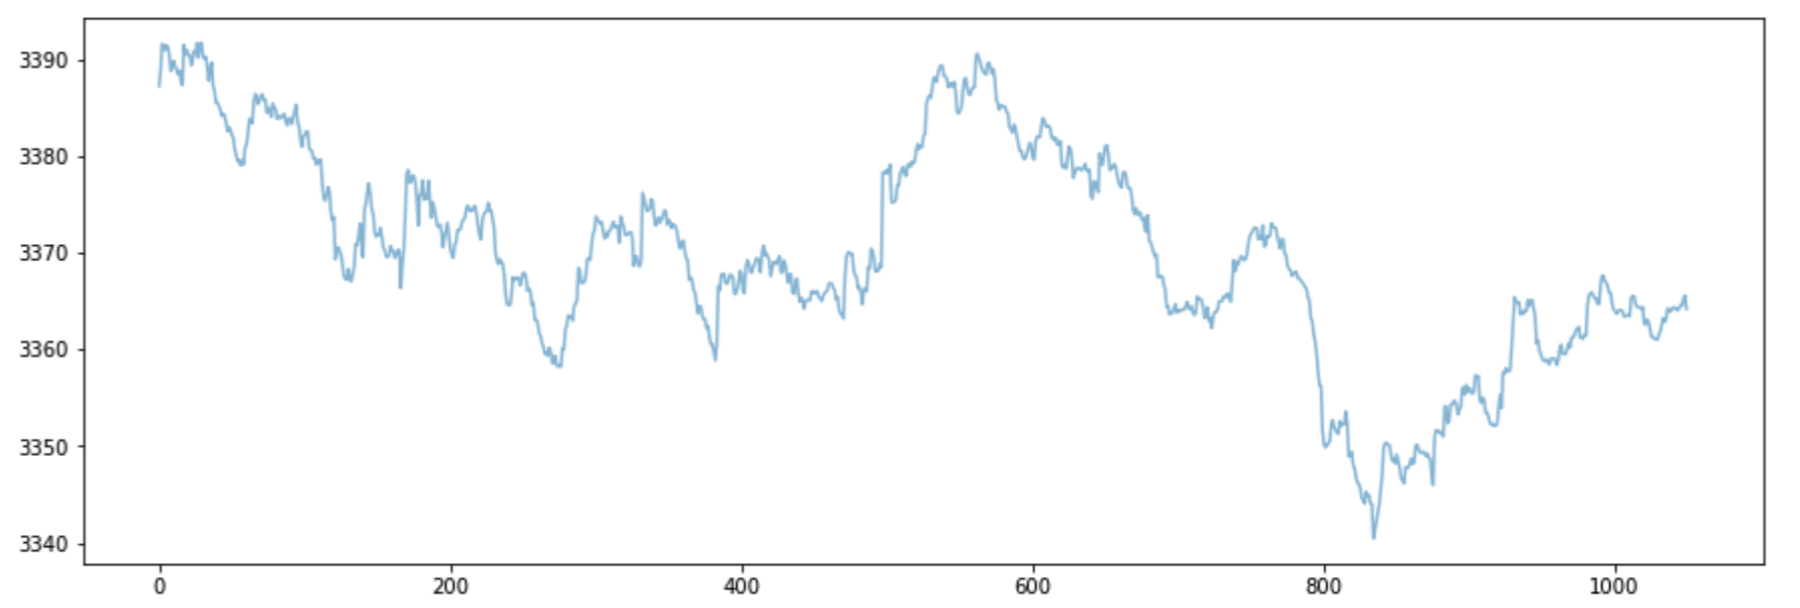
\includegraphics[width=0.42\textwidth]{./images/stock_example.png}
        \label{fig:stock}
        \caption{An Example of Stock Price Fluctuations Over Time}
    \end{center}
\end{figure}



\begin{figure}[!ht]
    \begin{center}
        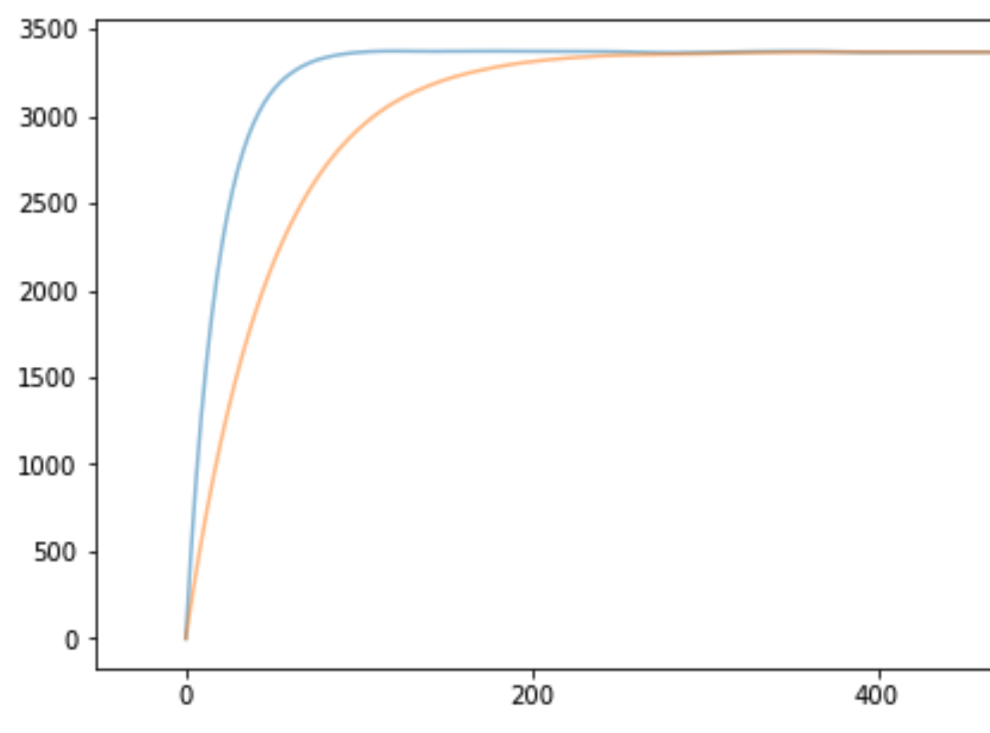
\includegraphics[width=0.42\textwidth]{./images/query2_example_200.png}
        \label{fig:EMA200}
        \caption{Exponential Moving Average of 38 and 100}
    \end{center}
\end{figure}



\begin{figure}[!ht]
    \begin{center}
        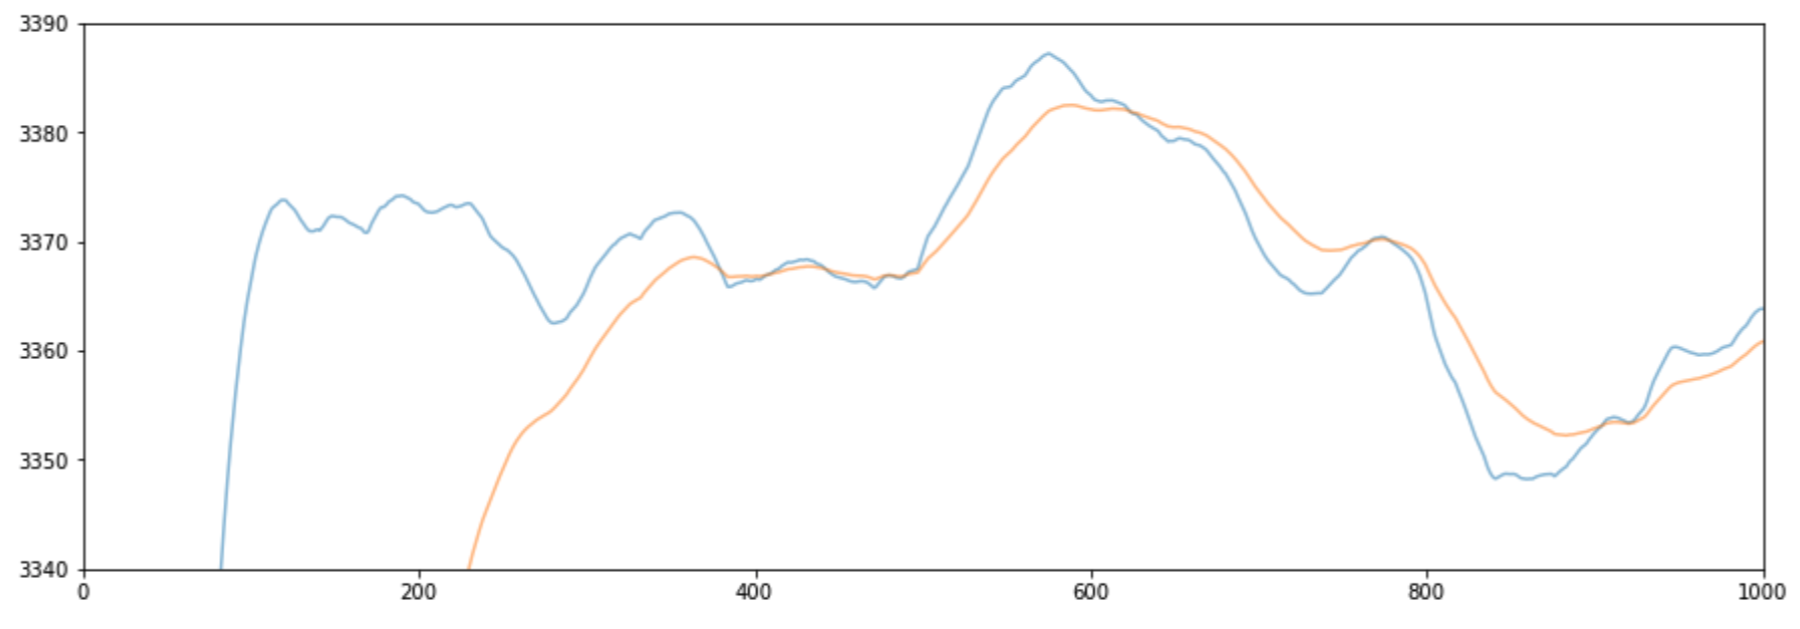
\includegraphics[width=0.42\textwidth]{./images/query2_example.png}
        \label{fig:EMAs}
        \caption{Example of Query 2 - Buy and Sell advice based on Breakout Patterns of EMA 38 and 100 }
    \end{center}
\end{figure}
